\documentclass{report}
\usepackage{amssymb, amsmath}
\usepackage{graphicx}
\usepackage{float}

\title{Examen Segundo Parcial}
\date{20 de Octubre de 2022}
\author{Nestor Adrian Sandoval Ortiz}

\begin{document}
    \maketitle
    \chapter{Funciones monovariables}
        \paragraph{Introduccion}
        Introduccion aqui

        \pagebreak

        \section{Primer Ejercicio}
            \begin{equation*}
                f(x)=x^2exp(x)+y^2exp(y)+1 
            \end{equation*}

            \begin{figure}[H]
                \includegraphics[width=\linewidth]{/Users/lloydna/Desktop/UP/5° Semestre/Optimizacion/Optimizacion/Examenes/Examen2/Ejercicio1/funcion.png}
                \caption{Grafica de la funcion y su minimo}
                \label{fig:fun11}
            \end{figure}

            \subsection{Tabla de resultados}
                \begin{tabular}{l|c|c|c|c|c|c}
                    & (x,y) Promedio & f(x,y) Promedio & Mejor (x,y) & Mejor f(x,y) & Peor (x,y) & Peor f(x,y)\\
                    \hline
                    Newton Raphson & (0.0, 0.0) & 1.0 & (0.0, 0.0) & 1.0 & (0.0, 0.0) & 1.0\\
                    \hline
                \end{tabular}
        \pagebreak

        \section{Segundo Ejercicio}
            \begin{equation*}
                f(x)=120+1.5x+\frac{0.2}{x}(1000) 
            \end{equation*}

            \begin{figure}[H]
                \includegraphics[width=\linewidth]{/Users/lloydna/Desktop/UP/5° Semestre/Optimizacion/Optimizacion/Examenes/Examen2/Ejercicio2/funcion.png}
                \caption{Grafica de la funcion y su minimo}
                \label{fig:fun12}
            \end{figure}

            \subsection{Tabla de resultados}
                \begin{tabular}{l|c|c|c|c|c|c}
                    & x Promedio & f(x) Promedio & Mejor x & Mejor f(x) & Peor x & Peor f(x)\\
                    \hline
                    Newton Raphson & 11.54348 & 154.64102 & 11.54348 & 154.64102 & 11.54348 & 154.64102\\
                    \hline
                \end{tabular}
        \pagebreak

        \section{Tercer Ejercicio}
            \begin{equation*}
                f(x)=x^2+x^4
            \end{equation*}

            \begin{figure}[H]
                \includegraphics[width=\linewidth]{/Users/lloydna/Desktop/UP/5° Semestre/Optimizacion/Optimizacion/Examenes/Examen2/Ejercicio3/funcion.png}
                \caption{Grafica de la funcion y su minimo}
                \label{fig:fun13}
            \end{figure}

            \subsection{Tabla de resultados}
                \begin{tabular}{l|c|c|c|c|c|c}
                    & x Promedio & f(x) Promedio & Mejor x & Mejor f(x) & Peor x & Peor f(x)\\
                    \hline
                    Newton Raphson & -0.0 & 0.0 & -0.0 & 0.0 & -0.0 & 0.0\\
                    \hline
                    Secante & -0.01295 & 0.00017 & -0.01295 & 0.00017 & -0.01295 & 0.00017\\
                    \hline
                \end{tabular}
        \pagebreak

        \section{Cuarto Ejercicio}
            \begin{equation*}
                f(x)=x^2+x^4
            \end{equation*}

            \begin{figure}[H]
                \includegraphics[width=\linewidth]{/Users/lloydna/Desktop/UP/5° Semestre/Optimizacion/Optimizacion/Examenes/Examen2/Ejercicio3/funcion.png}
                \caption{Grafica de la funcion y su minimo}
                \label{fig:fun14}
            \end{figure}

            \subsection{Tabla de resultados}
                \begin{tabular}{l|c|c|c|c|c|c}
                    & x Promedio & f(x) Promedio & Mejor x & Mejor f(x) & Peor x & Peor f(x)\\
                    \hline
                    Newton Raphson & -0.0 & 0.0 & -0.0 & 0.0 & -0.0 & 0.0\\
                    \hline
                    Secante & -0.01295 & 0.00017 & -0.01295 & 0.00017 & -0.01295 & 0.00017\\
                    \hline
                \end{tabular}
        \pagebreak

        \section{Quinto Ejercicio}
            \begin{equation*}
                f(x,y)=x^2+y^2-2x
            \end{equation*}

            \begin{figure}[H]
                \includegraphics[width=\linewidth]{/Users/lloydna/Desktop/UP/5° Semestre/Optimizacion/Optimizacion/Examenes/Examen2/Ejercicio5/funcion.png}
                \caption{Grafica de la funcion y su minimo}
                \label{fig:fun15}
            \end{figure}

            \subsection{Tabla de resultados}
                \begin{tabular}{l|c|c|c|c|c|c}
                    & (x,y) Promedio & f(x,y) Promedio & Mejor (x,y) & Mejor f(x,y) & Peor (x,y) & Peor f(x,y)\\
                    \hline
                    Newton Raphson (multidimensional) & (1.00001, 1.0e-5) & -1.0 & (1.00001, 1.0e-5) & -1.0 & (1.00001, 1.0e-5) & -1.0\\
                    \hline
                    Newton Raphson (unidimensional) & & & & & & \\
                    \hline
                    Secante (unidimensional) & & & & & & \\
                    \hline
                \end{tabular}
        \pagebreak

        \section{Sexto Ejercicio}
            \begin{equation*}
                f(x,y)=(x+2y-7)^2+(2x+y-5)^2
            \end{equation*}

            \begin{figure}[H]
                \includegraphics[width=\linewidth]{/Users/lloydna/Desktop/UP/5° Semestre/Optimizacion/Optimizacion/Examenes/Examen2/Ejercicio6/funcion.png}
                \caption{Grafica de la funcion y su minimo}
                \label{fig:fun16}
            \end{figure}

            \subsection{Tabla de resultados}
                \begin{tabular}{l|c|c|c|c|c|c}
                    & (x,y) Promedio & f(x,y) Promedio & Mejor (x,y) & Mejor f(x,y) & Peor (x,y) & Peor f(x,y)\\
                    \hline
                    Newton Raphson & (1.00001, 1.0e-5) & -1.0 & (1.00001, 1.0e-5) & -1.0 & (1.00001, 1.0e-5) & -1.0\\
                    \hline
                \end{tabular}
        \pagebreak

        \section{Septimo Ejercicio}
            \begin{equation*}
                f(X)=(100(X_{2}-X_{1}^2))^2+(1-X_{1})^2+90(X_{4}-X_{3}^2)^2+(1-X_{3})^2+10.1((X_{2}-1)^2+(X_{4}-1)^2)+19.8(X_{2}-1)(X_{4}-1)
            \end{equation*}

            \begin{figure}[H]
                \includegraphics[width=\linewidth]{/Users/lloydna/Desktop/UP/5° Semestre/Optimizacion/Optimizacion/Examenes/Examen2/Ejercicio6/funcion.png}
                \caption{Grafica de la funcion y su minimo}
                \label{fig:fun17}
            \end{figure}

            \subsection{Tabla de resultados}
                \begin{tabular}{l|c|c|c|c|c|c}
                    & X Promedio & f(X) Promedio & Mejor (X) & Mejor f(X) & Peor (X) & Peor f(X)\\
                    \hline
                    Gradiente & (0.99141, 0.98288, 1.00851, 1.01712) & 0.00026 & (0.99141, 0.98288, 1.00851, 1.01712) & 0.00026 & (0.99141, 0.98288, 1.00851, 1.01712) & 0.00026\\
                    \hline
                \end{tabular}
        \pagebreak
        
\end{document}